\documentclass{article}

% Language setting
% Replace `english' with e.g. `spanish' to change the document language
\usepackage[english]{babel}

% Set page size and margins
% Replace `letterpaper' with`a4paper' for UK/EU standard size
\usepackage[letterpaper,top=2cm,bottom=2cm,left=3cm,right=3cm,marginparwidth=1.75cm]{geometry}

% Useful packages
\usepackage{amsmath}
\usepackage{graphicx}
\usepackage[colorlinks=true, allcolors=blue]{hyperref}
\usepackage{algpseudocode}

\title{Global minimum/maximum using Enforced Hill Climbing Algorithm}
\author{Buțco George}
\date{}

\newcommand{\smallSpace}{\vspace{0.3cm}}
\newcommand{\mediumSpace}{\vspace{0.5cm}}

\algnewcommand\algorithmicforeach{\textbf{for each}}
\algdef{S}[FOR]{ForEach}[1]{\algorithmicforeach\ #1\ \algorithmicdo}

\begin{document}
\maketitle

\section{Introduction}

\textbf{Hill Climbing} is an \textbf{heuristic algorithm} used in numerical analysis. This algorithm is used to find the global minimum or maximum of a function. It uses incremental changes and if a change is better then the original value, it becomes the new solution.

This relative simple algorithm can be used for problems such as \textbf{Travelling Salesman Problem}.

\mediumSpace

\textbf{Enforced Hill Climbing} is a Hill Climbing Algorithm Variant witch uses \textbf{Breadth-first search} to not get stuck in a local optimum.

\section{Implementation}

\subsection{Pseudo Code}

\begin{algorithm}
\caption{Enforced Hill Climbing}\label{alg:cap}
\begin{algorithmic}
\State open-queue $ \gets $ [initial-vector]
\State best $ \gets $ f(initial-vector)

\While{\texttt{(list is not empty)}}

    \State current-vector $ \gets $ \texttt{pop vector from open-queue}
    \State successors $ \gets $ \texttt{list of vectors visible from the current-vector}
    \ForEach {next-vector $ \in $ successors}
        \State next-vector-value $ \gets $ f(next-vector)
        \If{(next-vector-value is better than best)}
            \State \texttt{clear successors}
            \State \texttt{clear open-queue}
            \State best $\gets$ next-vector-value
        \EndIf
        \State \texttt{push next-vector in open-queue}
    \EndFor
    
\EndWhile
\end{algorithmic}
\end{algorithm}

\newpage
\subsection{Successors Optimization}
An approach can be to create the successors list from incrementing in every direction from the current-vector.

This naive approach for finding the "neighbours" will check the same vector many times being hard to check vectors that are far from the current solution.

\begin{center}

\includegraphics[width=5cm]{latex_src/naive.png}
\end{center}

\mediumSpace

\textbf{A good approach can be:}

Defining an axis vector as a tuple (value, index, direction)

\smallSpace

Axis Vector = \begin{cases}
\texttt{value} = [x_0, x_1, \hdots x_k \hdots x_{n-1}] & k, n \in \mathbb{N}, k < n, n \geq 1
\\
\texttt{index} = k & k \in \mathbb{N}, k < n
\\
\texttt{direction} = -1 \texttt{ or } 1 \texttt{ (positive or negative)}
\end{cases}

\smallSpace

The successors of an Axis Vector are:

\smallSpace

\begin{cases}
[v_0, v_1, v_2], k < n-1
\\
[v_0], k = n-1
\end{cases}

\smallSpace

$v_0$ = \begin{cases}
\texttt{value} = [x_0, x_1, \hdots (x_k + step \cdot direction) \hdots x_{n-1}]
\\
\texttt{index} = k
\\
\texttt{direction} = \texttt{direction of the current vector}
\end{cases}

$v_1$ =  \begin{cases}
\texttt{value} = [x_0, x_1, \hdots x_k, (x_{k+1} + step) \hdots x_{n-1}]
\\
\texttt{index} = k+1
\\
\texttt{direction} = 1
\end{cases}


$v_2$ =  \begin{cases}
\texttt{value} = [x_0, x_1, \hdots x_k, (x_{k+1} - step) \hdots x_{n-1}]
\\
\texttt{index} = k+1
\\
\texttt{direction} = -1
\end{cases}

\begin{center}
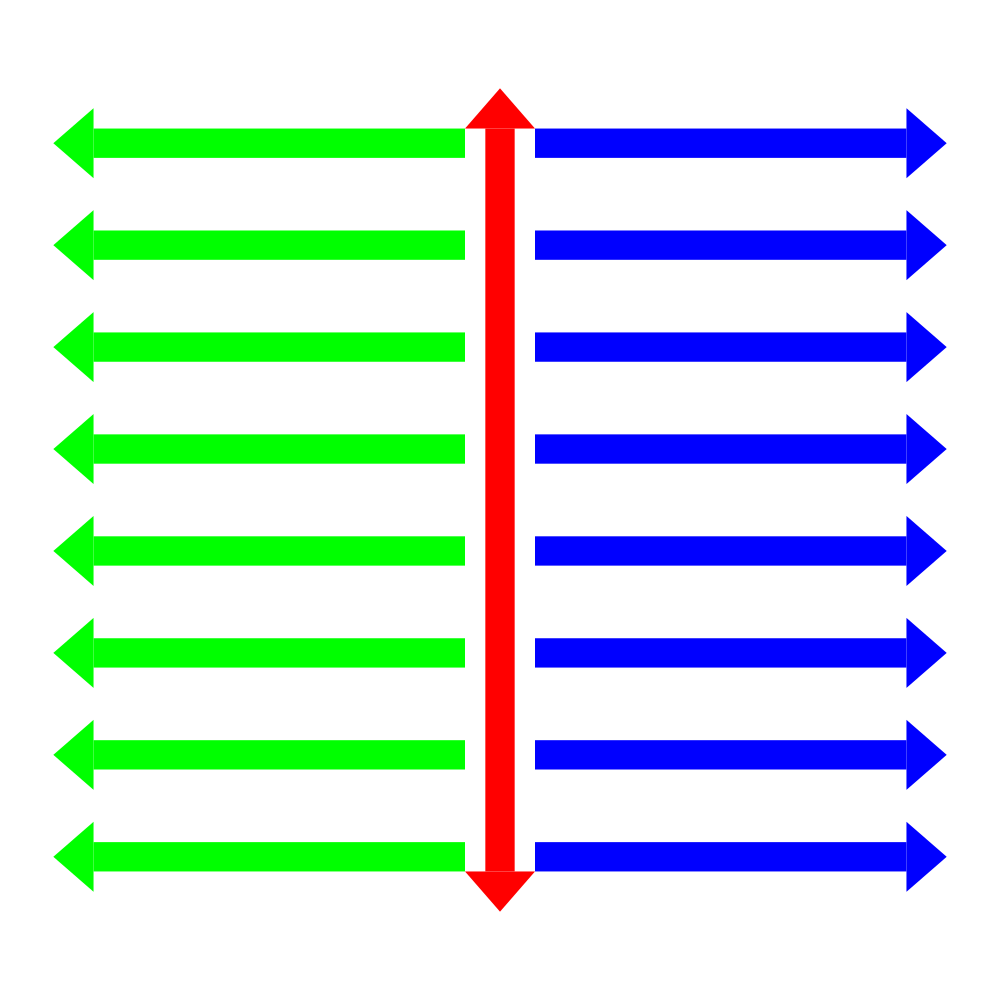
\includegraphics[width=5cm]{latex_src/good.png}
\end{center}

\subsection{C++ Implementation}
\href{https://github.com/George-debug/Uni-projects/tree/main/GA/T0/hillClimbingEnforced}{Link to GitHub folder}

\subsection{Testing}

\begin{itemize}
  \item
    Gramacy & Lee Function:
    \begin{center}
    $$\frac{sin(10 \pi x)}{2x}+(x-1)^4$$
    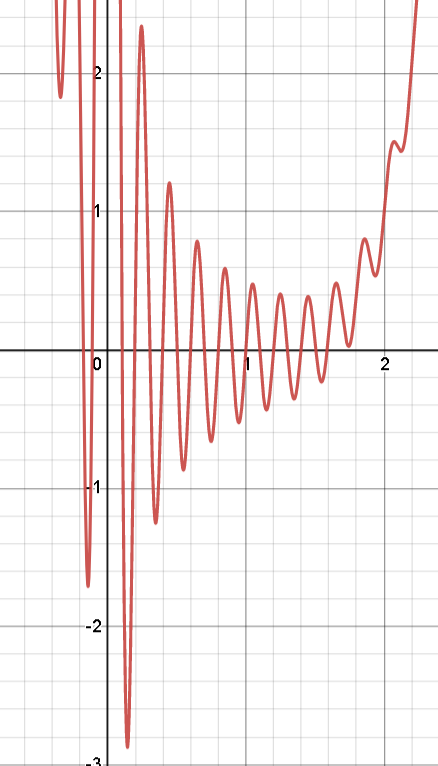
\includegraphics[height=5cm]{latex_src/GramacyLee.png}
    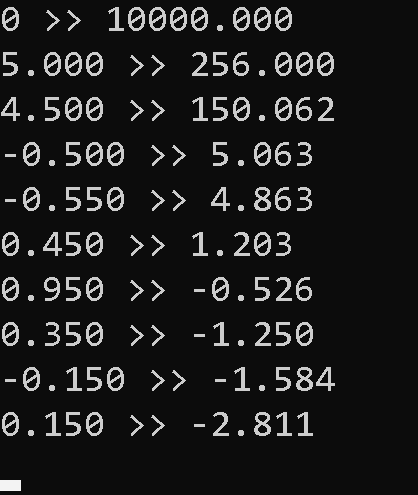
\includegraphics[height=5cm]{latex_src/gramacyLeeTest.png}
    \end{center}
  \item
     Heart Function:
    \begin{center}
     $$x^2 + \left( \frac{3y}{2} - \frac{x ^ 2 + abs(x) - 6}{x ^ 2 + abs(x) + 2}\right) ^ 2 - 36$$
    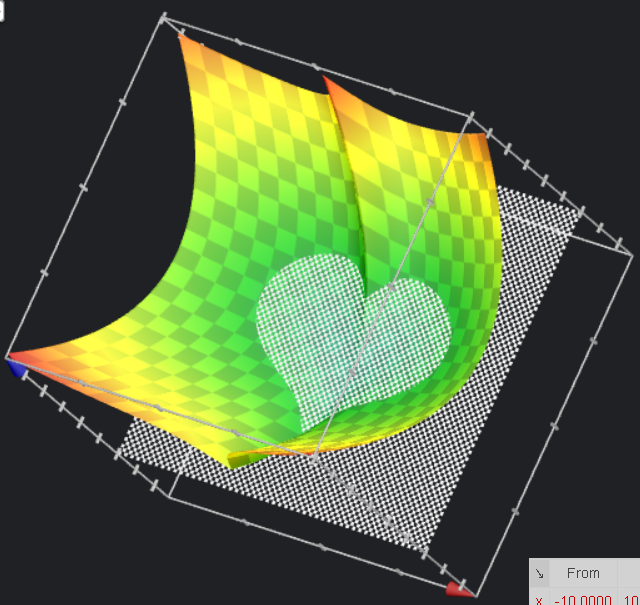
\includegraphics[height=5cm]{latex_src/heart.png}
    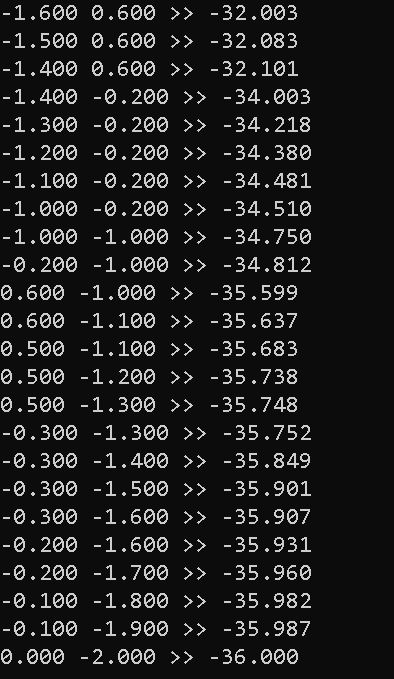
\includegraphics[height=5cm]{latex_src/heartTest.png}
    \end{center}
\end{itemize}

\end{document}